\documentclass{report}

% Matemática
\usepackage{amsmath}    % símbolos matemáticos
\usepackage{amsthm}     % teoremas
\usepackage{amsfonts}   % \mathbb
\usepackage{bm}         % bold math (https://ctan.org/pkg/bm)
\usepackage{abraces}    % \aunderbrace y \aoverbrace
\usepackage{mathtools}  % \mathclap

% Figuras
\usepackage{tikz}                   % gráficos
\usepackage{float}                  % [H]
\usepackage{xcolor}                 % colores https://es.overleaf.com/learn/latex/Using_colours_in_LaTeX

\usepackage{framed}     % textbars
% Texto
\usepackage[shortlabels]{enumitem}  % enumerate con letras

% Referencias
\usepackage[colorlinks=true]{hyperref}

\usetikzlibrary{arrows,positioning,automata,shadows,fit,shapes}

% Teoremas, corolarios, etc.
% https://www.overleaf.com/learn/latex/theorems_and_proofs
\theoremstyle{definition} % Para que no salga en italicas

\newtheorem{theorem}{Teorema}[chapter]
\newtheorem*{theorem*}{Teorema}

\newtheorem{lemma}{Lema}[chapter]
\newtheorem*{lemma*}{Lema}

\newtheorem{proposition}{Prop.}[chapter]
\newtheorem*{proposition*}{Prop}

\newtheorem{definition}{Def.}[chapter]
\newtheorem*{definition*}{Def}

\newtheorem{exmp}{Ejemplo}[chapter]
\newtheorem*{exmp*}{Ejemplo}

% https://tex.stackexchange.com/questions/118173/how-to-write-ceil-and-floor-in-latex
\DeclarePairedDelimiter\ceil{\lceil}{\rceil}
\DeclarePairedDelimiter\floor{\lfloor}{\rfloor}

% Comandos de AAA
\newcommand{\sigmatsequence}{\overset{\rightarrow}{\sigma}}
\newcommand{\tautsequence}{\overset{\rightarrow}{\tau}}

% Entornos
\newenvironment{nota}[1]
    {\begin{leftbar}\textbf{#1}}
    {\end{leftbar}}

\author{Manuel Panichelli}
\title{Notas de \\\textit{Algoritmos, Azar y Autómatas}}

\begin{document}

\maketitle

\chapter{Normalidad}

\section{Azar}

Azar es \textbf{imposibilidad de predecir}, \textbf{falta de patrones},
imposibilidad de abreviar, comprimir.

Vamos a categorizar el azar según diferentes modelos de cómputo

\begin{itemize}
    \item Autómatas finitos
    \item Autómatas de pila
    \item Máquinas de turing
\end{itemize}

\begin{definition}
    Una secuencia es \textbf{azarosa} (para los autómatas de la clase $C$)
    cuando, esencialmente, la única forma de describirla (mediante un autómata
    de la clase $C$) es nombrando explícitamente cada uno de sus símbolos.
\end{definition}

Esto quiere decir que no tiene patrones (porque sino podríamos nombrar menos) y
que no se puede comprimir. \textit{Esencialmente} porque se pueden hacer
pequeñas conversiones. Por ejemplo, las cadenas de $\{a^n b^n \mid n \in
\mathbb{N}\}$ son azarosas para AF pero no para AP (porque es un lenguaje libre
de contexto pero no regular).

Hay distintos \textit{grados de azar}:

\begin{enumerate}
    \item \textbf{Azar puro}: Impredecibilidad / incompresibilidad para
    máquinas de turing
    \item \textbf{Azar básico}: Impredicibilidad / incompresibilidad para
    autómatas finitos.
\end{enumerate}

\begin{enumerate}
    \item Una secuencia es \textbf{random} si, esencialmente, sus
    \textit{segmentos iniciales} solo se pueden describir explícitamente por una
    Turing Machine (no pueden ser comprimidos por una TM)
    \item Una secuencia es \textbf{normal} si, esencialmente, sus segmentos
    iniciales solo se pueden describir explicitamente por un autómata finito.
\end{enumerate}

Cosas que no copié

\begin{enumerate}
    \item Kolmogorov / program size complexity
    \item Definicion de azar de Chaitin basado en kolmogorov
    \item Martin Löf random
\end{enumerate}

\section{Numeros normales}

\begin{definition*}
    Una \textbf{base} es un entero $\geq 2$. Para un $x \in \mathbb{R}$ en el
    intervalo unitario\footnote{El intervalo unitario es el intervalo cerrado
    $[0, 1]$}, su \textbf{expansión} en base $b$ es una \textbf{secuencia} $a_1
    a_2 a_3 \dots$ de enteros de ${0, 1, \dots, b-1}$ tales que

    $$x = 0.a_1 a_2 a_3 \dots,$$

    donde $x = \sum_{k \geq 1} \frac{a_k}{b_k}$ y $x$ no termina con una cola de
    $b - 1$ (esto lo hacemos para tener una representación única de todos los
    numeros racionales)

    Cuando se de por sentada la base $b$ denotamos los primeros $n$ digitos de
    la expansión de $x$ con $x[1\dots n]$
\end{definition*}


\begin{definition}[Números normales, Borel 1909]\label{def:normal-borel}
    Un número real $x$ es,
    \begin{itemize}
        \item \textbf{Simplemente normal a base $b$} si en la expansión de $x$
        en base $b$, cada digito ocurre con una frecuencia de $1/b$ en el
        límite.

        $$\lim_{n\to \infty} \frac{|x[1\dots n|_d}{n} = \frac{1}{b}$$

        \textit{(En el límite todos los símbolos tienen la misma frecuencia)}
        \item \textbf{Normal a base $b$} si para cada entero positivo $k$, cada
        bloque de $k$ digitos (arrancando de cualquier posición) ocurre en la
        expansión de $x$ en base $b$ con una frecuencia en el límite de $1/b^k$
        \item \textbf{Absolutamente normal} si es normal para todas las bases.
    \end{itemize}
\end{definition}

\begin{exmp*} Algunos ejemplos son

    \begin{itemize}
        \item $0.01 \ 002 \ 0003 \ 00004 \ 000005 \ 0000006 \ 00000007 \ 000000008 \dots$
        no es simplemente normal a base $10$ (el 0 tiene más frecuencia que el
        resto)
        \item $0.0123456789 \ 0.0123456789 \ 0.0123456789 \ 0.0123456789 \dots$ es
        simpelemente normal a base $10$, pero no es simplemente normal a base 100.
    
        \textit{Pasar de base 10 a base 100 es tomar combinaciones de dos dígitos en base 10 de forma contigua}
    
        \item El ternario de cantor no es simplemente normal a base 3 (las
        expansiones no tienen el dígito 1)
    
        \item Los numeros racionales no son normales a ninguna base
        
        Si agarro un número racional, por ej 3.14
    
        $$3.14 \rightsquigarrow 3.140000000\dots$$
        
        en base 10 tiene un período que se repite
    
        \item La constante de Liouville $\sum_{n \geq 1} 10^{-n!}$ no es normal a
        base 10
    \end{itemize}    
\end{exmp*}


\begin{theorem}[Borel 1909]
    Casi todos los números reales son absolutamente normales.
\end{theorem}

Son las constantes matemáticas usuales como $\pi$, $e$ o $\sqrt{2}$
absolutamente normales? O al menos simplemente normales a alguna base? Es una
pregunta abierta.

\begin{theorem}[Champernowne, 1933]

    Todos los numeros naturales en base 10 concatenados es normal a base 10.

    $$0.123456789101112131415161718192021\dots$$

    \textit{No se sabe si es normal a bases que no son potencias de 10}
    
\end{theorem}

\begin{theorem}[Cassels 1959; Schmidth 1961]
    Casi todos los números del ternario de Cantor son normales a base 2.
\end{theorem}

\begin{theorem}[Bailey y Borwein 2012]
    El número de Stoneham $\alpha_{2, 3} = \sum_{k \geq 1} \frac{1}{3^k
    2^{3^k}}$ es normal a base 2 pero no simplemente normal a base 6.
\end{theorem}

\subsection{Normalidad y autómatas finitos}

\begin{definition}
    Una secuencia $x = a_1 a_2 a_3 \dots$ es \textbf{compresible} por un
    trasductor finito $T$ si y solo si en la corrida en $T$ $q_0
    \xrightarrow{a_1\mid v_1} q_1 \xrightarrow{a_2\mid v_2} q_2
    \xrightarrow{a_3\mid v_3} q_3 \dots$ satisface que

    $$\underset{n \to \infty}{\text{lim inf}}\ \frac{|v_1 v_2 \dots v_n|}{n} <
    1.$$
    
    \textit{Recordar que los $a$ son símbolols y los $v$ cadenas, posiblemente vacías.}
\end{definition}

\begin{theorem}
    Una secuencia es \textbf{normal} si y solo si es \textbf{incompresible por
    todo one-to-one transducer}.
\end{theorem}

\begin{theorem*}[Becher, Casrton, Heiber 2013]
    Los transductores finitos uno a uno no deterministicos con contadores no
    pueden comprimir secuencias normales.
\end{theorem*}

\begin{theorem*}
    
\end{theorem*}
    Los trasductores de pila no determinísticos pueden comprimir secuencias
    normales.
    
    $$
        0123456789\ \textcolor{blue}{9876543210}\
        00\ 01\ 02\ 03 \dots 98\ 99\ \textcolor{blue}{99\ 98\ 97 \dots 03\ 02\ 01\ 00\ }
        000\ 001\ 002 \dots
    $$

    \textit{Va pusheando y cuando detecta el cambio empieza a desapilar.
    Parecido al APD que reconoce $w\#w^r$}


\section{Notación}

\begin{itemize}
    \item Un \textit{alfabeto} es un conjunto finito de símbolos. Por ej $A$
    \item $A^\omega$ es el conjunto de todas las palabras infinitas
    \item $A^*$ (la clausura de Kleene) es el conjunto de todas las palabras finitas
    \item $A^{\leq k}$ es el conjunto de todas las palabras de longitud hasta $k$
    \item $A^{k}$ es el conjunto de palabras de longitud exactamente $k$.
    \item Si $w$ es una cadena $|w|$ es su longitud.
    \item Las posiciones de las cadenas se numeran desde 1
    \item $w[i]$ es el simbolo iésimo de $w$ y $w[i\dots j]$ es el substring de
    $i$ a $j$.
    \item La cadena vacía es $\lambda$
\end{itemize}

\begin{definition*}[Ocurrencia en cadena]
    Decimos que una palabra $u$ \textit{ocurre} en una cadena en una posición
    $i$ si $w[i\dots i+|u|-1] = u$. (\textit{omitimos decir ambas posiciones
    para las ocurrencias})
\end{definition*}


\begin{definition}[Ocurrencias alineadas y no alineadas]
    El número de ocurrencias alineadas y no alineadas de una cadena es

    \begin{align*}
        |w|_u &= |\{ i : w[i\dots i+|u| - 1] = u\}|,\\
        ||w||_u &= |\{ i : w[i\dots i+|u| - 1] = u \text{ y } i \equiv 1 \text{ mod } |u|\}|
    \end{align*}

    Cuando $u$ es un símbolo las definiciones coinciden. Y la de alineadas son
    posiciones que son múltiplos de $|u|$

    \textit{(La de alineadas tiene $\equiv 1$ en vez de $\equiv 0$ ya que las posiciones se numeran de 1)}
    
    \begin{exmp*}
        $|aaaaa|_{aa} = 4$ y $||aaaaa||_{aa} = 2$.
    \end{exmp*}

\end{definition}

\begin{proposition*}
    Las ocurrencias alineadas de una palabra de longitud $r$ sobre un alfabeto
    $A$ coinciden con las ocurrencias del símbolo correspondiente sobre el
    alfabeto $A^r$.
\end{proposition*}
\begin{proof}
    Sean un alfabeto $A$, una longitud $r$ y un alfabeto $B$ con $|A|^r$
    símbolos (la cantidad de símbolos que tiene el alfabeto $A^r$). $A^r$ (el
    conjunto de palabras de longitud $r$ sobre el alfabeto $A$) y $B$ son
    isomorfos, existe

    $$\pi: A^r \to B$$

    que se induce del orden lexicográfico en cada conjunto (se puede hacer un
    matching 1 a 1). Por lo tanto, para cada $w \in A^*$ tal que $|w|$ es
    múltiplo de $r$,

    $$|\pi(w)| = |w| / r.$$

    (Una palabra de longitud múltiplo de $r$ es una cadena de $r$ símbolos de
    $A^r$, luego la longitud de la palabra en $B$ que tiene símbolos unitarios
    digamos es esa).

    Luego,

    $$\forall u \in A^r \ (||w||_u = |\pi(w)|_{\pi(u)}).$$
\end{proof}

Por ejemplo, sean $A = \{0, 1\}$, $r = 3$, y $B$ tal que $|A^r| = |B|$,

$$B = \{
    \underset{000}{0},
    \underset{001}{1},
    \underset{010}{2},
    \underset{011}{3},
    \underset{100}{4},
    \underset{101}{5},
    \underset{110}{6},
    \underset{111}{7}
\}$$

Luego la cadena,

$$100\ 100\ 111\ 000$$
$$4470$$

La cantidad de ocurrencias de $100$ coinciden con las de $4$.

\begin{definition}[Normalidad no alineada, Borel]
    Un número real $x$ es \textbf{normal a base $\bm{b}$} si para cada bloque
    $u$,

    $$
    \underset{n \to \infty}{lim}
        \frac{|x[1\dots n]|_u}{n} =
        \frac{1}{b^{|u|}}.
    $$

    \textit{En el límite,como $b^{|u|}$ son todos los bloques posibles de
    longitud $|u|$, $1/b^{|u|}$ seria que cada uno tiene la misma frecuencia.}
\end{definition}

\begin{theorem}[Piatetski-Shapiro]\label{teo:piatetski-shapiro}
    Sea $x$ un número real, $b \geq 2$ un entero y $A = \{0, \dots, b - 1\}$.
    Las siguientes son equivalentes
    \begin{enumerate}
        \item $x$ es normal a base $b$
        \item Existe una constante $C$ tal que para infinitas longitudes $\ell$ y
        para todo $w \in A^\ell$

        $$
            \limsup_{n\to\infty}
            \frac{||x[1\dots n\ell]||_w}{n} < C \cdot b^{-\ell}.
        $$ 

        \item Existe una constante $C$ tal que para infinitas longitudes $\ell$ y
        para todo $w \in A^\ell$

        $$
            \limsup_{n\to\infty}
            \frac{|x[1\dots n]|_w}{n} < C \cdot b^{-\ell}.
        $$
    \end{enumerate}
\end{theorem}

\begin{proof}[Dem 3 $\Rightarrow$ 1]
    \textit{Para el ejercicio 4 hay que hacer la 2da.}

    Sea $x$ un número real. Queremos llegar a \nameref{def:norm-non-aligned}, para cada bloque $u$

    $$\lim_{n\to \infty} \frac{|x[1\dots n]|_u}{n} = \frac{1}{|u|}.$$

    Sabemos que se cumple 3, es decir que existe una constante $C$ tal que para
    toda longitud $\ell$ y $w \in A^\ell$,

    $$
    \limsup_{n\to\infty}
    \frac{|x[1\dots n]|_w}{n} < C \cdot b^{-\ell}.
    $$

    Observemos que para todo $w \in A^*$, $n$ y $k$, para contar las ocurrencias
    de $w$ en $x[1\dots nk]$ puedo contar las ocurrencias en todas las sub
    palabras de longitud $k$. En total puede ocurrir a lo sumo $k - \ell + 1$ veces.

    \[
        |x[1\dots nk]|_w
            \geq \frac{1}{k - \ell + 1} \sum_{v \in A^k} |x[1\dots nk]|_v |v|_w.
    \]

    \begin{figure}[H]
        \centering
        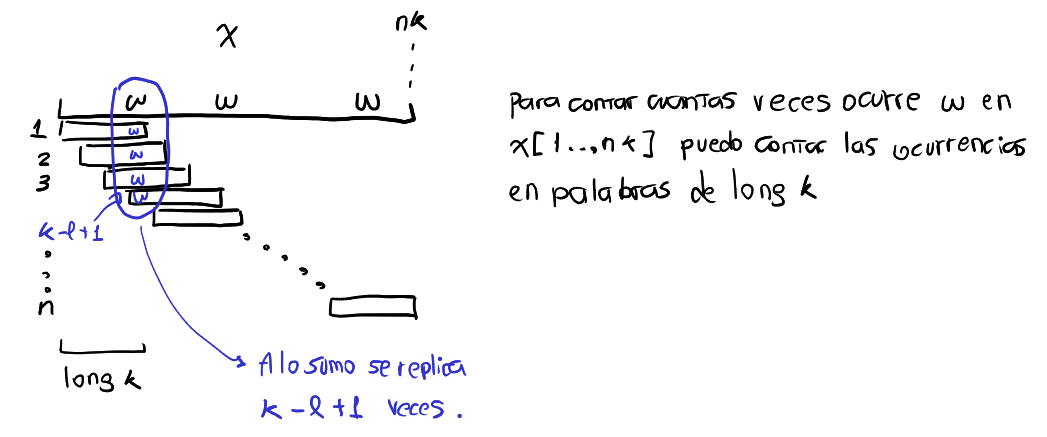
\includegraphics[scale=0.3]{img/3_pts.png}
    \end{figure}

    Como sabemos algo del lim sup, y queremos usar \nameref{prop:lim-trick},
    arrancamos con lim inf.

    \begin{align*}
        \liminf_{n\to \infty} \frac{|x[1\dots nk]_w}{nk}
            &\geq
                \liminf_{n\to \infty}
                \frac{1}{k - \ell + 1} 
                    \sum_{v \in A^k} \frac{|x[1\dots nk]|_v}{nk} |v|_w \\
            &\geq
                \liminf_{n\to \infty}
                \frac{1}{k} 
                    \sum_{v \in A^k} \frac{|x[1\dots nk]|_v}{nk} |v|_w 
            &&(\ell + 1 \geq 0)\\
            &= \liminf_{n\to \infty}
                \sum_{v \in A^k} \frac{|x[1\dots nk]|_v}{nk} \frac{|v|_w}{k}
    \end{align*}

    Supongamos que existe $C$ tal que para longitudes infinitas $\ell$ y para
    todo $w \in A^\ell$

    $$
    \limsup_{n\to\infty}
    \frac{|x[1\dots n]|_w}{n} < C \cdot b^{-\ell}.
    $$

    Sea $k$ una de esas longitudes. Fijamos $\epsilon \leq 1/b^{\ell}$, $w
    \in A^\ell$. Sea $k$ suficientementer grande para que $|Bad(A, k, w,
    \epsilon)| < b^k \epsilon$

    \begin{align*}
        \liminf_{n\to \infty}
            \sum_{v \in A^k}
            \aunderbrace[l1r]{\frac{|x[1\dots nk]|_v}{nk} \frac{|v|_w}{k}}_{K}
        &= \liminf_{n\to \infty}
            \sum_{v \in A^k \setminus Bad(A, k, w, \epsilon)} K
        &&\text{(separo en bad y no bad)} \\
        &+ \liminf_{n\to \infty}
        \sum_{v \in A^k \cap Bad(A, k, w, \epsilon)} K \\
        &\geq \liminf_{n\to \infty}
        \sum_{v \in A^k \setminus Bad(A, k, w, \epsilon)} K
        &&\text{(no cuento las malas)}
    \end{align*}

    Y como $v \notin Bad(A, k, w, \epsilon) \Rightarrow \frac{|v|_w}{k} \geq
    b^{-|w|} \pm \epsilon$
    
    % https://tex.stackexchange.com/questions/91505/how-to-extend-the-text-under-summation-symbol-without-making-extra-space
    \begin{align*}
        \liminf_{n\to \infty}
        \sum_{\mathclap{v \in A^k \setminus Bad(A, k, w, \epsilon)}}
            \frac{|x[1\dots nk]|_v}{nk} \frac{|v|_w}{k}
        &\geq (1 - \epsilon) b^{-\ell}\ \liminf_{n\to \infty}
            \sum_{\mathclap{v \in A^k \setminus Bad(A, k, w, \epsilon)}}
            \frac{|x[1\dots nk]|_v}{nk} \\
        &= (1 - \epsilon) b^{-\ell}\ \liminf_{n\to \infty}
        \left( 1 -\sum_{v \in Bad(A, k, w, \epsilon)}
        \frac{|x[1\dots nk]|_v}{nk} \right)
        && (\sum \text{good} = 1 - \sum \text{bad}) \\
        &\geq (1 - \epsilon) b^{-\ell}\
            \left( 1 -
                \sum_{v \in Bad(A, k, w, \epsilon)}
                \limsup_{n\to \infty}
                \frac{|x[1\dots nk]|_v}{nk}
            \right)\\
        &\geq (1 - \epsilon) b^{-\ell}\
        \left( 1 -
            \sum_{v \in Bad(A, k, w, \epsilon)} C \cdot b^{-k}
        \right) \\
        &\geq (1 - \varepsilon) b^{-\ell}(1 - C\varepsilon)
        &&(|Bad(A, k, w, \epsilon)| < b^k \epsilon)
    \end{align*}

    Y como es cierto para todo $\varepsilon \geq b^{-\ell}$ positivo, podemos tomar
    un $\varepsilon$ suficientemente chico para que $(1 - \varepsilon)
    b^{-\ell}(1 - C\varepsilon) \approx b^{-\ell}$

    % Por qué vale???
    % (1 - \epsilon) b^{-\ell}(1 - C\epsilon)
    % = b^{-\ell} (1 - C\epsilon - \epsilon + C \epsilon^2)

    % 1 - C\epsilon - \epsilon + C \epsilon^2 = 1
    % <=> - C\epsilon - \epsilon + C \epsilon^2 = 0
    % <=>  C \epsilon^2 = C\epsilon + \epsilon
    % <=>  C \epsilon^2 = (C + 1) \epsilon
    % <=>  C \epsilon = C + 1
    % <=>  \epsilon = 1 + 1/C

    $$\liminf_{n\to \infty} \frac{|x[1\dots nk]|_w}{nk} \geq b^{-\ell}.$$

    Finalmente, por el lemma \nameref{prop:lim-trick} y como es cierto para todo
    $w \in A^\ell$,

    $$\lim_{n \to \infty} \frac{|x[1\dots n]|_w}{n} = b^{-\ell}$$

    y concluyo que $x$ es normal.
\end{proof}



\section{Tres secuencias normales}

\begin{itemize}
    \item Secuencias de Bruijn infinitas
    \item A la Champernowne (binario)
    
    $$01\ \ 00\ 01\ 10\ 11\ \ 000\ 001\ 010\ 011\ 100\ 101\ 110\ 111\ \ 0000 \dots$$

    \item Una secuencia normal tal que la subsecuencia en las posiciones pares
    es idéntica a toda la secuencia.
\end{itemize}

\section{De Bruijn}

\begin{definition}[De Bruijn 1946]
    Definiciones de De Bruijn,
    \begin{itemize}
        \item Un \textbf{collar de De Bruijn} de orden $n$ sobre un alfabeto $A$
        es una secuencia cíclica de longitud $|A|^n$ tal que cada palabra de
        longitud $n$ ocurre en ella exactamente una vez.

        Ejemplos: 01; 0011; 00011101 (el 100 está en la pos 8 por ej.).

        \item Una \textbf{palabra de De Bruijn} (no cíclica) de orden $n$ sobre
        el alfabeto $A$ es una palabra de longitud $|A|^n + n - 1$ (se le agrega
        todo lo que uno podría hacer con un ciclo, desde la última posición una palabra con longitud $n$ podría llegar hasta $n-1$ más al principio) tal que cada palabra de
        longitud $n$ ocurre en ella exactamente una vez.

        Ejemplos: 01; 00110; 0001110100.

        \item Una \textbf{palabra infinita de De Bruijn} $w = a_1 a_2 \dots$ en
        un alfabeto de al menos tres símbolos es una palabra infinita tal que,

        $$\forall{n}.\ a_1\dots a_{|A|^n + n - 1}$$

        es una palabra de De Bruijn de orden $n$.

        Ejemplo: 012, una palabra de De Bruijn de orden 1, se puede extender a
        la siguiente de orden 2: 0122002110.

        Si el alfabeto tiene dos símbolos, una palabra infinita de De Bruijn $w
        = a_1 a_2 \dots$ es aquella que para cada $n$ impar, $a_1\dots a_{|A|^n
        + n - 1}$ es una palabra de De Bruijn de orden $n$.
    \end{itemize}
\end{definition}

\begin{definition}
    Un \textbf{grafo de De Bruijn} $G_A(n)$ es un digrafo cuyos vértices son
    palabras de longitud $n$ sobre el alfabeto $A$ y sus ejes los pares $(au,
    ub)$ para alguna palabra $u$ de longitud $n - 1$ y posiblemente dos símbolos
    diferentes $a, b$.

    \begin{figure}[H]
        \centering
        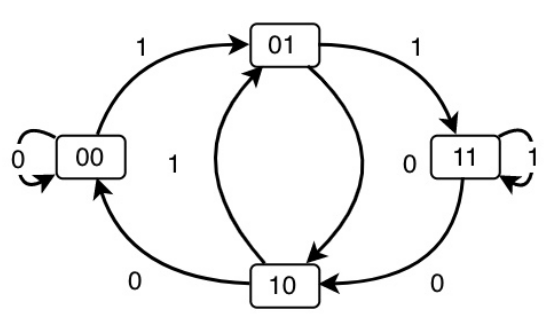
\includegraphics[scale=0.3]{img/2_de_brujin_01.png}
        \caption{Ejemplo de grafo de De Bruijn de orden 2 para $A = \{0, 1\}$}
    \end{figure}
    
    \begin{itemize}
        \item Tiene $|A|^n$ vertices y $|A|^{n+1}$ arcos
        \item Es \textit{fuertemente conexo} (existe un camino dirigido entre
        todo par de vértices)\footnote{Conexo a secas en digrafos es que el grafo
        subyacente (sacándole direcicones) sea conexo}
        \item Es \textit{regular}, $\forall v. d_{in}(v) = d_{out}(v)$ (los
        loops suman uno a la entrada y salida)
        \item Es Euleriano (por teorema de Euler, solo hace falta que sea
        regular y fuertemente conexo).
    \end{itemize}
\end{definition}

\begin{figure}[H]
    \centering
    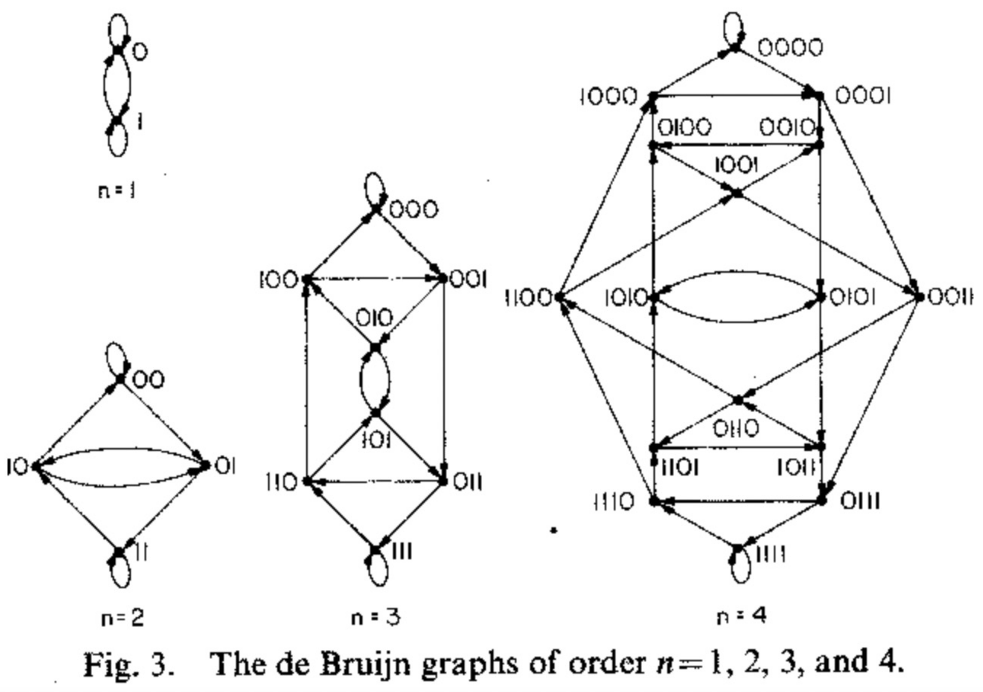
\includegraphics[scale=0.3]{img/2_de_brujin_ord_1234.png}
    \caption{Grafos de De Bruijn de ordenes 1, 2, 3 y 4 sobre $A = \{0, 1\}$}
\end{figure}

\begin{definition*}
    El \textbf{grafo de línea} de un grafo $G$, es otro grafo que tiene como
    vértilos ejes de $G$ y como ejes los caminos de longitud 2.
\end{definition*}


\begin{proposition}
    Toda secuencia de De Bruijn de orden $n+1$ sobre un alfabeto de $|A|$
    simbolos se puede construir como un ciclo Euleriano en $G_A(n)$.
\end{proposition}

\begin{proposition}[Becher, Heiber 2011]\label{prop:de-brujin-extend}
    Dado un alfabeto $A$ con al menos tres símbolos, toda secuencia de De
    Bruijn de orden $n$ se puede extender a una de orden $n + 1$
\end{proposition}
\begin{proof}
    Dado un alfabeto $A$, suponiendo que $E$ es un ciclo Euleriano de $G_A(n)$.
    Como $G_A(n + 1)$ es el grafo de línea de $G_A(n)$, $E$ es un ciclo
    Hamiltoniano en $G_A(n+1)$.

    \textit{Todo ciclo euleriano va a ser hamiltoniano en el grafo de línea, 
    porque los vertices son los ejes}
    
    \textit{\textcolor{blue}{Está la demo completa en las clases, no la terminé
    de ver.}}

\end{proof}

Para computar una palabra infinita de De Bruijn puedo para cada $n \geq 1$
extender un ciclo Hamiltoniano en un grafo de De Bruijn de orden $n$ a uno
Euleriano en el mismo grafo. Esto se hace en tiempo exponencial de $n$, y no se
conoce ningun algoritmo eficiente.

\begin{theorem}[Ugalde 2000]
    Las palabras infinitas de De Bruijn son normales.

    Si el alfabeto $A$ tiene dos símbolos, se puede considerar el alfabeto $A'$
    de 4 símbolos que se obtiene con el morfismo que mapea bloques de dos
    simbolos en $A$ a un simbolo en $A'$ y probar normalidad ahí.
\end{theorem}
\begin{proof}[Dem.]
    Intuitivamente, una secuencia es normal si cada bloque de dígitos ocurre con
    la misma frencuencia en el límite que cada otro bloque de la misma longitud
    (ver Def \nameref{def:normal-borel}). Para probarlo, el numero de ocurrencias en
    una posición arbitraria está acotado por el numero de ocurrencias al final
    del megabloque.
    
    \begin{figure}[H]
        \centering
        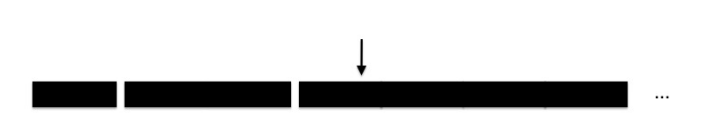
\includegraphics[scale=0.3]{img/2_de_brujin_inf_normal_block.png}
    \end{figure}

    Quiero ver que las palabras infinitas de De Bruijn son normales. Sea $\ell$ una longitud cualquiera, $u \in A^\ell$ un bloque de esa longitud y $n > |A|^\ell + \ell - 1$ ($u$ pertenecerá a una palabra de De Bruijn de orden $\ell$, que tiene longitud $|A|^\ell + \ell - 1$).

    $u$ ocurre en una palabra de De Bruijn de orden $n$ entre $|A|^{n - \ell}$
    y $|A|^{n - \ell} + n - \ell$ veces
    \begin{itemize}
        \item Aparece al menos $|A|^{n - \ell}$ veces porque como en una palabra de De Bruijn de orden $n$ aparecen todas las cadenas de tamaño $n$ una vez, el bloque $u$ va a aparecer con $|A|^{n - \ell}$ terminaciones distintas.
        
        En otras palabras, hay exactamente $|A|^{n - \ell}$ palabras de longitud $n$ que tienen como primeros $\ell$ símbolos a $u$.

        \begin{figure}[H]
            \centering
            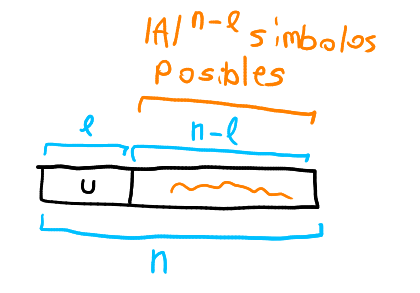
\includegraphics[scale=0.3]{img/2_de-brujin-normal-inf.png}
        \end{figure}

        \item A lo sumo $|A|^{n - \ell} + n - \ell$ porque hay exactamente $n - \ell$ posiciones en una palabra de De Bruijn de orden $n$ en las cuales podría comenzar una palabra de longitud $\ell$. \textcolor{red}{no me termina de quedar claro}
    \end{itemize}

    Sea $x = a_1 a_2 \dots$ una palabra infinita de De Bruijn sobre A. Por definición, para cada $n$

    $$a_1\dots a_{|A|^n + n - 1}$$

    es una palabra de De Bruijn de orden $n$. Fijemos $N$ una posición en la palabra infinita que esté entre el final de la palabra de De Bruijn de orden $n$ y $n+1$,
    
    $$|A|^n + n - 1 \leq N < |A|^{n+1} + n.$$

    Luego,

    \begin{align*}
        \frac{|a_1\dots a_N|_u}{N} &\leq
        \frac{|a_1\dots a_{|A|^{n+1} + n}|_u}{|A|^n + n - 1} &\text{(Por la cota que define N)} \\
        &\leq \frac{|A|^{n+1 - \ell} + n - 1}{|A|^n + n - 1}
        & \text{(\#ap de u en De Bruijn de orden n + 1)}\\
        &< 2 |A|^{-\ell + 1}. &\text{(cuentita)}
    \end{align*}

    Por lo tanto,

    \[
        \underset{N \to \infty}{\text{lim sup }} \frac{|a_1\dots a_N|_u}{N}
        < 2 |A|^{-\ell + 1}.
    \]

    El Teorema \nameref{teo:piatetski-shapiro} nos dice que un número real $x$
    es normal para una base $b$ si existe una constante $C$ tal que para
    infinitas longitudes $\ell$ y para todo $w \in A^\ell$

    $$
        \underset{n \to \infty}{\text{lim sum}}
        \frac{|x[1\dots n]|_w}{n} < C \cdot b^{-\ell}.
    $$

    Interpretado para cadenas, podemos decir que $b$ es el tamaño del alfabeto y
    que la expansión hasta $n$ es un bloque de tamaño $n$. Por lo tanto, tomando
    $b = |A|$ y $C = 2|A|$ se cumple y concluimos que $x$ (una palabra infinita
    de De Bruijn) es normal.
\end{proof}

\section{Collares perfectos (\textit{Perfect Necklaces})}

Consideremos todos los bloques de tamaño $n$, concatenados en orden
lexicografico y vistos circularmente (como \textit{collares}). Cada bloque de
tamaño $n$ ocurre exactamente $n$ veces en posiciones diferentes modulo $n$.

Por ejemplo, para el alfabeto $\{0, 1\}$ y $n = 2$, los bloques concatenados en orden lexicográfico son $00\ 01\ 10\ 11$ y

% Lo dejo acá solamente porque estaba quedando fachero.
% \begin{align*}
%     &\overset{1}{0}
%     \overset{2}{0}\
%     \overset{3}{0}
%     \overset{4}{1}\
%     \overset{5}{1}
%     \overset{6}{0}\
%     \overset{7}{1}
%     \overset{8}{1} \\
%     &00\ 01\ 10\ 11 \\
%     &00\ 01\ 10\ 11 \\
%     &00\ 01\ 10\ 11 \\
%     &00\ 01\ 10\ 11 \\
%     &00\ 01\ 10\ 11 \\
%     &00\ 01\ 10\ 11 \\
%     &00\ 01\ 10\ 11 \\
% \end{align*}

\begin{figure}[H]
    \centering
    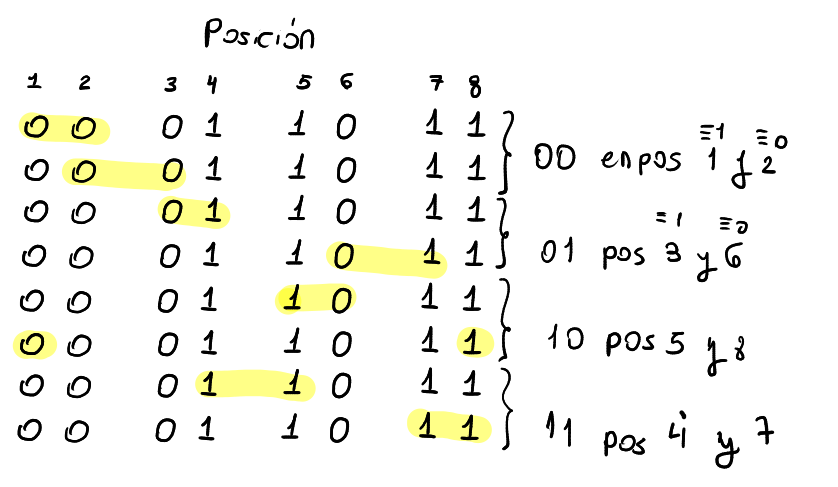
\includegraphics[scale=0.3]{img/2_perf-neckl-2.png}
\end{figure}

No toda permutación de los bloques de longitud $n$ tiene esta propiedad, por ejemplo

\begin{itemize}
    \item $\bm{00}\ 10\ 11\ 01$: El $00$ aparece solamente 1 vez.
    \item $\bm{000}\ 101\ 001\ 010\ 011\ 100\ 110\ 111$: El $000$ aparece solo una vez.
\end{itemize}

\begin{definition}[Collar perfecto]
    Un collar (cadena circular) sobre un alfabeto de $b$ símbolos se dice
    $\bm{(n, k)}$\textbf{-perfecto} si cada bloque de longitud $n$ ocurre $k$
    veces, en posiciones diferentes modulo $k$, para cualquier convención de
    punto de partida.
\end{definition}

Observaciones:

\begin{itemize}
    \item Los collaras de De Bruijn son exactamente los collares $(n, 1)$-perfectos.
    \item Los collares $(n, k)$-perfectos tienen longitud $k b^n$
\end{itemize}

\section{Definiciones equivalentes de normalidad}

Un número real $x$ es \textbf{simplemente normal en base b} si en la expansión
de $x$ en base $b$ cada digito $d$ ocurre con frecuencia $1/b$ en el límite,

$$\lim_{n\to\infty} \frac{|x[1\dots n]|_d}{n} = \frac{1}{b}$$

\begin{definition}[Strong aligned normality]\label{def:norm-strong-aligned}
    \textit{(Borel 1909)}
    
    Un numero real $x$ es \textbf{normal en base b} si cada real $x, bx, b^2 x,
    \dots$ son simplemente normales a las bases $b^1, b^2, b^3, \dots$

    \textit{$bx$ es shiftear a la izquierda, correr la coma y tirar el 1er símbolo. $b^2x$ es lo mismo pero tirando dos símbolos y quedándose con el resto.}
\end{definition}

\begin{definition}[Aligned normality]\label{def:norm-aligned}
    \textit{(Pillai 1940)}.
    
    Un número real $x$ es \textbf{normal en base b} si $x$ es simplemente normal en bases $b^1, b^2, b^3, \dots$

    \textit{No hacen falta los shifts, esto es como tomar alineada.}
\end{definition}

\begin{definition}[Non-aligned normality]\label{def:norm-non-aligned}
    \textit{(Nivel and Zuckerman 1951)}
    
    Un número real $x$ es \textbf{normal en base b} si para cada bloque $u$,

    $$\lim_{n\to\infty} \frac{|x[1\dots n]|_u}{n} = \frac{1}{|u|}$$
\end{definition}

\begin{theorem}
    Las tres definiciones de normalidad son equivalentes.
\end{theorem}

\begin{proof} Vamos a probar que
    \nameref{def:norm-strong-aligned}
    $\Rightarrow$ \nameref{def:norm-non-aligned}
    $\Rightarrow$ \nameref{def:norm-aligned}
    $\Rightarrow$ \nameref{def:norm-strong-aligned}
\begin{enumerate}
    \item \nameref{def:norm-strong-aligned} 
    $\Rightarrow$ \nameref{def:norm-non-aligned}

    Por la definición de normalidad alineada furte, sabemos que dado número $x$
    cada real $b^i x$ es simplemente normal a base $b^i$, es decir que para cada
    dígito $w$ con $\ell = |w|$ y para cada $i$,
    
    % https://tex.stackexchange.com/questions/17528/show-equation-number-only-once-in-align-environment
    \begin{align}
        \lim_{n\to \infty} \frac{\|(b^ix)[1\dots\ell n]\|_w}{n} = b^{-\ell}
        &\Leftrightarrow \lim_{n\to \infty} \frac{\|(b^ix)[1\dots n]\|_w}{n/\ell} = b^{-\ell} \nonumber \\
        &\Leftrightarrow \lim_{n\to \infty} \frac{\|(b^ix)[1\dots n]\|_w}{n} = b^{-\ell}/\ell. \label{teo:norm-eq-1}
    \end{align}

    Para cualquier $w \in A^\ell$, contar de manera no alineada es lo mismo que
    de forma alineada con todos los shifts ($n - i$ porque no me puedo pasar)
    
    $$|x[1\dots n]|_w = \sum_{i=0}^{\ell - 1} \|(b^ix)[1\dots n - i]\|_w.$$

    Luego,

    \begin{align*}
        \lim_{n\to \infty} \frac{|x[1\dots n|_w}{n}
            &= \lim_{n\to \infty}
                \sum_{i=0}^{\ell - 1} \|(b^ix)[1\dots n - i]\|_w \\
            &= \sum_{i=0}^{\ell - 1} 
                \lim_{n\to \infty} \|(b^ix)[1\dots n - i]\|_w \\
            &= \sum_{i=0}^{\ell - 1} 
                b^{-\ell}/\ell = b^{-\ell}
    \end{align*}

    Y por lo tanto es normal de forma no alineada.

    \item \nameref{def:norm-non-aligned} $\Rightarrow$ \nameref{def:norm-aligned}
    
    \textit{En clase}

    \item \nameref{def:norm-aligned} $\Rightarrow$ \nameref{def:norm-strong-aligned}

    \textit{En clase}

\end{enumerate}
\end{proof}

\subsection{Malas palabras}

Intuitivamente, un segmento inicial se comporta bien o mal con respecto a lo que
espero en el límite? Bien sería que se parezca, por ej. 1/2 de 1s y 1/2 de 0s.
Mal sería que tenga más 0s que 1s.

\begin{definition*}[Malas palabras]
    Sean $A$ un alfabeto de $b$ simbolos, $k$ un entero positivo y $\epsilon$ un
    real entre 0 y 1. Definimos el conjunto de palabras de longitud $k$ tales
    que una palabra $w$ tiene un número de ocurrencias que difiere de lo
    esperado $\pm \epsilon k$,

    $$Bad(A, k, w, \epsilon) = \left\{
        v \in A^k : 
            \left|
                |v|_w -
                \frac{k}{b^{|w|}}
            \right| > \epsilon k
    \right\}.$$

    Donde $|v|_w$ es lo \textit{observado} y $\frac{k}{b^{|w|}}$ es lo
    \textit{esperado}
\end{definition*}
\begin{exmp*} Por ejemplo,
    \begin{itemize}
        \item $A = \{ 0, 1 \}, k = 4, \epsilon = 1/4, w = 11$.
        
        Tenemos lo esperado $\frac{k}{b^{|w|}} = \frac{4}{2^2} = 1$, y la
        tolerancia $\epsilon k = 1$.
        Entonces $Bad(A, k, w, \epsilon) = \{1111\}$ es el conjunto de palabras
        con 3 ocurrencias de $w$ (no alineadas).

        \item $A = \{ 0, 1 \}, k = 4, \epsilon = 1/4, w = 1$.

        Tenemos $\frac{k}{b^{|w|}} = \frac{4}{2^1} = 2, \epsilon k = 1$.
        Entonces $Bad(A, k, w, \epsilon) = \{1111, 0000\}$ es el conjunto de palabras
        con 4, 0 ocurrencias de $w$.
    \end{itemize}
\end{exmp*}

Los siguientes teoremas muestran que hay pocas malas palabras

\begin{lemma}[Hardy and Wright, Theorem 148]\label{lemma:bad-digit-bound}
    Sean $b \geq 2$ y $k \geq 0$ enteros. Si $6/k \leq \epsilon \leq 1/b$
    entonces para cada \textbf{símbolo} $d$ en $A$,

    $$|Bad(A, k, d, \epsilon)| < 4e^{-b\epsilon^2 k/6}b^k.$$
\end{lemma}

\textit{Obs para ejercicio 4: puedo ver dígitos en el alfabeto $A^k$ para long $k$, y ahí estoy viendo ocurrencias alineadas.}

\begin{lemma}
    Sea $A$ un alfabeto de $b$ símbolos, $k, \ell$ enteros positivos y
    $\epsilon$ un real tal que $6/\floor{k / \ell} \leq \epsilon \leq 1/b^\ell$.
    Entonces,

    $$\left| \bigcup_{w \in A^\ell} Bad(A, k, w, \epsilon) \right|
    < 2\ell\ b^{2\ell}\ e^{-b^\ell \epsilon^2k/(6\ell)}b^k.$$
\end{lemma}

\begin{theorem}
    Casi todas las secuencias son normales
\end{theorem}
\begin{proof}
    En clase 3 diapo 18, usa Bad.
\end{proof}

\begin{lemma}[Pequeño truco de límites]\label{prop:lim-trick}
    \textit{Relación entre lim inf / lim sup y lim}


    Sean $(x_{1, n})_{n\geq0}, (x_{2, n})_{n\geq0},\dots (x_{k, n})_{n\geq0}$
    una secuencia de números reales tales que $\sum_{i=1}^{k} x_{i, n} = 1$ y
    $c_1, c_2, \dots c_k$ numeros reales tales que $\sum_{i=1}^{k} c_i = 1$.
    Luego,
    
    \begin{enumerate}
        \item $\forall i\ \liminf_{n\to \infty} x_{i, n} \geq c_i
        \implies \forall i\ \lim_{n\to \infty} x_{i, n} = c_i$

        \item $\forall i\ \limsup_{n\to \infty} x_{i, n} \leq c_i
        \implies \forall i\ \lim_{n\to \infty} x_{i, n} = c_i$
    \end{enumerate}

    Vamos a aplicar esto para $k = b^\ell$, 
    $x_{n, i} = \frac{|x[1..n]|_{w_i}}{b^\ell}$ con $i = 1, 2, \dots b^\ell$.
    
    Notar que
    
    $$\sum_{i=1}^{b^\ell} \frac{|x[1..n]|_{w_i}}{b^\ell} = 1,$$
    
    donde

    \begin{itemize}
        \item n = \# palabras de $\ell$ caracteres (n posiciones que quiero mirar)
        \item $w_i$ = palabras de longitud $\ell$
    \end{itemize}

    en total tengo $n$ ocurrencias. $\ell$ fijo y voy moviendo la posición. Es
    como un sliding window.

    % x[1 a \ell]
    % x[2 a \ell + 1]
    % x[3 a \ell + 2]
    % x[n - \ell a n]
    % x[n a n + \ell - 1]

    \textit{Supongo que es con x normal}
\end{lemma}
\begin{proof}[Dem]
    ``Puedo mirar las familias de lim inf y me alcanza para afirmar el límite".
    Es además un problema dual. Asumo 1. y veo que me da 2, el otro es análogo.
    % TODO: agregar anotaciones de por qué vale c/u.
    \begin{align*}
        \limsup_{n \to \infty} x_{i, n}
            &= \limsup_{n \to \infty}\ (1 - \sum_{j \neq i} x_{j, n})
            &&\text{(pues }\sum_{i=1}^{k} x_{i, n} = 1)\\
            &= 
                \aunderbrace[l1r]{\limsup_{n \to \infty} 1}_{=1} + 
                \limsup_{n \to \infty}\ (- \sum_{j \neq i} x_{j, n}) \\
            &= 1 - \liminf_{n \to \infty}\ \sum_{j \neq i} x_{j, n} \\
            &\leq 1 - \sum_{j \neq i} \liminf_{n \to \infty}\ x_{j, n} \\
            &\leq 1 - \sum_{j \neq i} c_j
            &&\text{(por hip. 2.\ }\liminf_{n \to \infty}\ x_{j, n} \geq c_i) \\
            &= c_i
            &&\text{(por hip.} \sum_{i = 1}^{k} c_i = 1)
    \end{align*}

    Y como
    $$\limsup_{n \to \infty} x_{i, n} \leq c_i \leq \liminf_{n \to \infty} x_{i,
    n}$$
    
    y lim sup $\geq$ lim inf, necesariamente

    $$\limsup_{n \to \infty} x_{i, n} = c_i = \liminf_{n \to \infty} x_{i,
    n}$$

    y entonces
    $$\lim_{n\to \infty} x_{i, n} = c_i.$$
\end{proof}

\section{Algoritmos para absoluta normalidad}

Un número $x$ es \textbf{absolutamente normal} si es normal para todas las
bases.

\begin{definition}[Número computable]
    Un número real $x$ es computable si hay un programa de computadora que tiene
    de output su expansión fraccionaria en alguna base, dígito por dígito.
\end{definition}


\begin{theorem}[Turing 1936]
    Sea $x$ un número real en el intervalo unitario ($[0, 1]$). Los siguientes
    son equivalentes:

    \begin{enumerate}
        \item $x$ es computable
        \item Existe uan función computable $f: \mathbb{N} \to \{0, 1\}$ tal que
        $f(n)$ es el n-ésimo dígito en la expansión fraccionaria de $x$ en base
        2.
        \item Hay una secuencia computable no decreciente de numeros racionales
        $(q_j)_{j \geq 1}$ tal que $\lim_{j \to \infty} q_j = x$ y para cada
        $j$, $|x - q_j| \leq 2^{-j}$

        \textit{Los primeros $j$ símbolos están bien, porque sino la resta no
        daría $\leq 2^{-j}$. Es como decir "presición j", todo lo que venga
        despu[es de la pos j son 0s y 1s.}

        \item Hay una secuencia computable de intervalos $I_1, I_2, I_3, \dots$
        con bordes racionales anidados, cuyas longitudes van a 0 de forma tal
        que $x \in \bigcap_{j\geq 1} I_j$.

        \textit{Por ejemplo $I_1$ puede ser $[0, 1]$, y luego $I_2$ tiene que estar anidado, por ejemplo la mitad. Y en el límite, en la intersección infinita está $x$.}
    \end{enumerate}
\end{theorem}

\begin{exmp*}
    Ejemplos son 0, $\sqrt{2}$, $\pi$, $e$. Y un contraejemplo es el
    argumento diagonal de Cantor (tengo un ejemplo en mis notas).
\end{exmp*}

\subsection{Algoritmo de Turing}

\begin{theorem*}[Turing 1937?]
    Hay un algoritmo que computa la expansión en base 2 de un número
    absolutamente normal en el intervalo unitario.
\end{theorem*}

El algoritmo usa intervalos diádicos (potencias de 2). Para seleccionar $I_1,
I_2, I_3, \dots$ la estrategia es ``seguir la medida". El número computado $x$
entonces es la traza de las elecciones left / right. La definción de normalidad
absoluta que usa es

\begin{definition*}[Normalidad absoluta]
    Un número real $x$ es absolutamente normal si es simplemente normal en todas
    las bases enteras $b \geq 2$.
\end{definition*}

\begin{definition*}[Discrepancia simple]
    Sean $x \in [0, 1]$ un real y $x_b$ su expansión en base $b$, definimos
    
    \[
        \Delta_N(x_b) = \max_{d \in \{ 0, \dots, b-1 \}}
        \left|
            \frac{|x_b[1\dots N]|_d}{N} - \frac{1}{b}
        \right|
    \]

    \textit{Es como el desvío máximo de la frecuencia de un dígito de lo esperado en el segmento inicial de tamaño N. Discrepancia simple. $\Delta_N(x_b)$ se dice el dígito con la peor proporción}

    Luego $x$ es simplemente normal en base $b$ si

    \[ \lim_{N \to \infty} \Delta_N(x_b) = 0 \]

\end{definition*}

\begin{definition*}[Pasos del algoritmo]
    Usamos $n$ como el paso del algoritmo y definimos las sig funciones,
    
    \begin{itemize}
        \item[] $\bm{N_n} = 2^{n_0 + 2n}$, el número de dígitos vistos en el paso
        $n$, donde $n_0 = 11$ (\textit{$n_0$ solo está ahí para simplificar las
        cuentas})
        
        \item[] $\bm{b_n} = \floor{\log{N_n}}$ es la base más grande considerada en
        el paso $n$

        \item[] $\bm{\epsilon_n} = 1/b_n$ es la diferencia entre la frecuencia
        esperada de dígitos y la frecuencia actual en el paso $n$. El
        \textit{nivel de tolerancia}, dependiente de la cantidad de bases que se
        están viendo.
    \end{itemize}

    $b_n \geq 2$ y es no decreciente y no acotada, $N_n$ es no decreciente y no
    acotada, y $\epsilon_n$ es no creciente y va a 0.
\end{definition*}

\begin{definition*}[Conjuntos de candidatos]
    Definimos los conjuntos de números reales

    \begin{align*}
        E_0 &= (0, 1) \\
        E_n &= \bigcap_{b \in \{ 2, \dots, b_n \} }
            \{ x \in (0, 1) : \Delta_{N_n} (x_b) < \epsilon_n \}
    \end{align*}

    Para cada $n$, el conjunto $E_n$ consiste de todos los números reales cuyas
    expansiones en las bases $2, 3, \dots, b_n$ exhiben \textbf{buenas
    frecuencias} de digitos hasta $\epsilon_n$, en los primeros $N_n$ digitos
    (en el segmento inicial de tamaño $N_n$)
\end{definition*}

\begin{lemma*}
    El conjunto $\bigcap_{n \geq 0} E_n$ tiene medida positiva y consiste de
    solo números absolutamente normales.
\end{lemma*}

El algoritmo en sí es

\begin{itemize}
    \item[] \textbf{Paso inicial,} \bm{$n = 0$}. $I_0 = (0, 1),\ E_0 = (0, 1)$
    \item[] \textbf{Paso recursivo,} \bm{$n > 1$}
    
        En el paso anterior computamos $I_{n - 1}$. Sea $I_n^0$ la mitad
        izquierda de $I_{n - 1}$ y $I_n^1$ la mitad derecha.
        \begin{itemize}
            \item Si $\mu \left( I_n^0 \cap \bigcap_{j = 0}^{n} E_j \right) >
            1/N_n$ entonces $I_n = I_n^0$ y $y_n = 0$.

            \textcolor{blue}{No entiendo la condición}

            \item Sino, $I_n = I_n^1$ y $y_n = 1$.
        \end{itemize}
        \textit{$\mu A = |A|$ es la medida de Lebesgue de A. La probabilidad de que un número real positivo arbitrario aparezca en eso}
\end{itemize}

El output es $y_1y_2y_3\dots$.

Es un algoritmo \textit{goloso}: Parte el intervalo obtenido en el paso anterior
a la mitad, y se queda con la mitad que tiene más números que empiecen bien. Si
elije el de la izq toma como dígito 0, y sino elige el de la der y toma 1.

\subsubsection{Demostración de correctitud de algoritmo de Turing}

\begin{proposition*}
    Para cada $n$, $E_n$ es una unión finita de intervalos abiertos con bordes
    racionales, y para $n \geq n_0$, $\mu E_n > 1 - \frac{1}{N^2_n}$.
\end{proposition*}
\begin{proof}[Dem]
    Los valores de $N_n$ y $\epsilon_n$ satisfacen las hipótesis del Lema
    \ref{lemma:bad-digit-bound}
\end{proof}

\begin{proposition*}
    
\end{proposition*}

\subsection{BHS}

\begin{definition*}[b-ario]
    Decimos que un intervalo es $b$-ario (o $b$-ádico) de orden $n$ si tiene la
    forma

    \[
        \left(\frac{a}{b^n}, \frac{a+1}{b^n}\right)
    \]

    para algun entero $a$ tal que $0 \leq a < b^n$.

    Si $\sigma_b$ y $\tau_b$ son intervalos $b$-arios y $\tau_b \subseteq
    \sigma_b$ decimos que el \textit{orden relativo} de $\tau_b$ con respecto a
    $\sigma_b$ es el orden de $\tau_b$ menos el orden de $\sigma_b$.
\end{definition*}

\begin{lemma}[Lemma 3.1 BHS 2013]
    Sean $u$ y $v$ bloques y $\varepsilon$ un real positivo,

    \begin{enumerate}
        \item Si $\Delta(u) < \varepsilon$ y $\Delta(v) < \varepsilon$ entonces
        $\Delta(uv) < \varepsilon$.

        \textit{Si u es buena y v también, entonces su concatenación lo es.
        Esto me dice que si cuento dígito, puedo considerar la suma de las
        proporciones y va a andar todo bien.}

        \item Si $\Delta(u) < \varepsilon, v = a_1 \dots a_{|v|}$ y $|v|/|u| <
        \varepsilon$ entonces $\Delta(vu) < 2\varepsilon$ y para cada $\ell$ tal
        que $1 \leq \ell \leq |v|, \Delta(ua_1a_2\dots a_l) < 2\varepsilon$.

        \textit{Concatenar una palabrita mucho mas chica que una buena al lado
        de una buena a lo sumo empeora el doble la discrepancia}.
        
        $|v|/|u| < \varepsilon \Leftrightarrow |v| < \varepsilon|u|$, y como
        $\varepsilon$ es un número chiquito entre 0 y 1, se interpreta como que
        $u$ es muy chica en comparación a $v$.

        Para el algoritmo, nos dice que lo que ya viste no hace falta volverlo a
        mirar, podés mirar cosas nuevas. Si tengo un buen segmento inicial y lo
        que elijo para agregar es cortito, a lo sumo llevo mi discrepancia al doble.
    \end{enumerate}
\end{lemma}

\begin{lemma}[Lemma 3.4 BHS2013]

    Para cualquier intervalo $I$ y cualquier base $b$, hay un subintervalo
    $b$-ario $J$ tal que $\mu J \geq \mu I / (2b)$.

    \textit{Podemos encontrar J grande y $b$-ádico que se parezca mucho en medida}
\end{lemma}
\begin{proof}
    La idea es que queremos que sea lo más grande posible, porque si es muy
    chico va a tener símbolos con muchos dígitos asociados como para mirar.
    Idealmente quiero un dígito por cada base para el algoritmo.

    Como $J$ es b-ádico, sabemos que para algún $a$

    $$J = \left(\frac{a}{b^n}, \frac{a+1}{b^n}\right),$$

    y luego

    \[
        \mu J = \frac{a+1}{b^n} - \frac{a}{b^n} = \frac{a - a + 1}{b^n} = \frac{1}{b^n} = b^{-n}
    \]

    Como $I$ no es exactamente b-ádico, hay dos casos,

    \begin{enumerate}
        \item J calza exactamente.
        \item J va a caballo de dos b-ádicos.
    \end{enumerate}

    \textit{más en las notas draft de la clase}
\end{proof}

\begin{definition*}[t-sequences]
    Una t-sequence $\sigmatsequence$ es una secuencia de intervalos $(\sigma_2,
    \dots, \sigma_t)$ tales que

    \begin{itemize}
        \item Para cada base $b = 2, \dots, t$, $\sigma_b$ es b-ario.
        \item Para cada base $b = 3, \dots, t$, $\sigma_b \subset \sigma_{b-1}$
        y $\mu \sigma_b \geq \mu \sigma_{b-1} / (2b)$.
    \end{itemize}

    \textit{Son intervalos anidados, con la medida lo más grande posible.}

    La definición implica que $\mu \sigma_t \geq (\mu \sigma_2)/(2^t t!)$
    \textit{(es un peor caso, no siempre ocurre y a veces calza justo)}
    \begin{nota}{Para el ejercicio 6}

        Como hay que hacer para bases 2 y 3, vamos a necesitar
    
        \[
            \sigma_2, \sigma_3, \sigma_{2^i}, \sigma_{3^i}
        \]
    
        (si se hace demás, no está mal pero hay que ser \textit{económicos})
    \end{nota}

\end{definition*}

\begin{definition*}[Refinamiento]
    Dos definiciones,

    \begin{itemize}
        \item Una $t$-sequence $\overset{\rightarrow}{\tau} = (\tau_2, \dots,
        \tau_t)$ \textit{refina} una $t'$-secuencia $\sigmatsequence = (\sigma_2,
        \dots, \sigma_{t'})$ si $t' \leq t$ y $\tau_b \subset \sigma_b$ para cada
        $b = 2, \dots, t'$.

        \item Un refinamiento tiene \textit{discrepancia} menor a $\varepsilon$
        si para cada $b = 2, \dots, t'$ hay palabras $u, v$ tales que $\sigma_b
        = I_u, \tau_b = I_{uv}$ y $\Delta(v) < \varepsilon$.
    \end{itemize}
    

    \textit{El $\tau$ que elegiste tiene una discrepancia $< \varepsilon$.}
\end{definition*}

\begin{lemma}\label{lemma:bhs-refinement}
    Sean $t \geq 2$ un entero, $t' = t \vee t + 1$, $\varepsilon < 1/t$ un real
    positivo. Luego, toda $t$-sequence $\sigmatsequence = (\sigma_2, \dots,
    \sigma_t)$ admite un refinamiento $\tautsequence = (\tau_2, \dots,
    tau_{t'})$ con discrepancia menor a $\varepsilon$.

    El orden relativo de $\tau_2$ puede ser cualquier entero $k$ tal que
    
    \[
        k \geq max
        \left\{
            \frac{6}{\varepsilon},
            \frac{24(\log_2 t)(\log(t!))}{\varepsilon^2}
        \right\}.
    \]
\end{lemma}
\begin{proof}[Dem.]
    En clase diapo 5.
\end{proof}

\begin{definition*}[Pasos del algoritmo]
    El algoritmo considera las siguientes funciones para un paso $n$ dado,
    
    \begin{itemize}
        \item[] $\bm{t_n} = \max(2, \floor{\sqrt[4]{\log n}})$ es la máxima base
        a considerar en el paso $n$,
        \item[] $\bm{\varepsilon_n} = 1/t_n$ es la discrepancia máxima tolerada
        en el paso $n$, y
        \item[] $\bm{N_n} = \floor{\log n} + n_{\text{start}}$ es el número de
        dígitos en base 2 agregados en el paso $n$,
    \end{itemize}

    Donde $n_{\text{start}}$ es el minimo entero que valida la condición del
    Lema \ref{lemma:bhs-refinement}. Por lo tanto, requerimos que para todo $n >
    0$,
    
    \[
        \floor{\log n} + n_{\text{start}} \geq max
        \left\{
            \frac{6}{\varepsilon},
            \frac{24(\log_2 t)(\log(t!))}{\varepsilon^2}
        \right\}.
    \]
    
\end{definition*}

El algoritmo construye $\sigmatsequence_0, \sigmatsequence_1, \sigmatsequence_2,
\dots$ tal que $\sigmatsequence_0 = (0, 1)$ y para cada $n \geq 1$,
$\sigmatsequence_n$ es una $t_n$-sequencia que refina $\sigmatsequence_{n-1}$
con discrepancia $\varepsilon_n$ y tal que el orden de $\sigma_{n, 2}$ es $N_n$
mas el orden de $\sigma_{n-1}, 2$.

Tiene de output $x = y_1 y_2 y_3\dots$ que son los símbolos en la expansión en
base 2 de un número absolutamente normal.

\begin{itemize}
    \item[] \textbf{Paso inicial,}\bm{$n = 1$}. 
        $\sigmatsequence_1 = (\sigma_2)$, con $sigma_2 = (0, 1)$.
    \item[] \textbf{Paso recursivo,} \bm{$n > 1$}
    
        En el paso anterior computamos 
        $\sigmatsequence_{n-1} = (\sigma_2, \dots, \sigma_{t_n - 1})$.

        Tomamos $\sigma_n = (\tau_2, \dots, \tau_{t_n})$ la $t_n$-sequence más a
        la izquierda que refina $\sigmatsequence_{n-1}$ con discrepancia menor
        que $\varepsilon_n$ tal que si $\sigma_2 = I_u$ entonces $\tau_2 =
        I_{uv}$ con $|v| = N_n$.

        Ponemos $y_{M_n + 1}\dots y_{M_n + N_n} = v$ donde $M_n = \sum_{j =
        1}^{n} N_n$.
\end{itemize}
\begin{proof}
    En clase diapo 13.
\end{proof}

\end{document}
